%%!TEX root = diss.tex

\chapter{From particle dynamics to the sediment flux}
\label{ch:flux}
\section{Introduction}

A relativity weak flow shearing a bed of sediment entrains individual particles into a state of motion controlled by turbulent forcing and intermittent collisions with other grains at rest on the bed, generating wide fluctuations in the sediment velocity \citep{Heyman2016,Fathel2015}.
Bed load particles move downstream until they are disentrained when they happen to encounter sufficiently sheltered pockets on the bed surface to interrupt their motions \citep{Charru2004,Gordon1972}.
Eventually, the bed around them rearranges and destroys this shelter, or turbulent fluctuations overcome the shelter \citep{Celik2014,Valyrakis2010}, particles are once again entrained, and the cycle repeats.
Bed load transport is thus a kind of itinerant motion, characterized by alternation between fluctuating movements and rest.
This process is difficult to describe mathematically given the technicality of the stochastic physics involved \citep{Furbish2017,Ancey2020}.

To date, descriptions of bed load transport have therefore simplified the problem in various ways to enable progress.
The foundational work is due to Einstein, who considering bed load motions as instantaneous so he could describe bed load transport as an alternating sequence of ``steps" and rests having random length and duration \citep{Einstein1937}, in a pioneering application of the continuous time random walk \citep{Montroll1965}.
Einstein concluded that particles move downstream with a mean velocity $\bra u \ket = k_E l$, where $k_E$ is the rate at which an individual bed particle entrains into motion, and $l$ is the mean length of each downstream step.
Later, Einstein applied these ideas to calculate the mean downstream flux due to the movements of many such particles \citep{Einstein1950}. Einstein reasoned that if the density of resting particles on the bed is $\rho_b$, the overall areal entrainment rate of particles can be written $E = \rho_b k_E$, giving a mean sediment flux $\bra q_s \ket = \rho_b \bra u \ket  = El $.

Many researchers have since refined Einstein's approach to provide more realistic descriptions of individual particle motions than Einstein's instantaneous step model.
One set of efforts has neglected particle deposition process to calculate the downstream velocity distributions of moving particles after entrainment using mechanistic equations with terms representing turbulent fluid forces and particle-bed collisions \citep{Ancey2014,Fan2014}. 
Another set of efforts has described particles alternating between motion and rest, considering that motions occur with a constant velocity \citep{Lisle1998,Lajeunesse2017,Pierce2020b}. 
No models have yet been formulated which describe particles alternating between motion and rest, while motions have a realistic fluctuating velocity.

A set of studies has developed stochastic formulations of the sediment flux which improve on the mean field description provided by Einstein \citep{Furbish2012}. 
Sediment fluxes generally exhibit wide fluctuations due to variations in the number of moving particles and their velocities \citep{Ancey2008,Ancey2014}, the migration of bedforms and sediment waves \citep{Hamamori1962,Guala2014,Hoey1992,Recking2012}, and a host of other processes \citep{Dhont2018}.
Because these fluctuations occur over disparate timescales, measurements of mean sediment fluxes depend on the timescale over which they are collected, a phenomenon called scale-dependence \citep{Saletti2015,Dhont2018,Singh2009,Turowski2010,Ancey2020}.
To date, very few models have calculated the probability distribution of the bed load sediment flux due to individual particle motions \citep{Ancey2008,Ancey2014}, and among these, even fewer have described any observation-scale dependence of the flux \citep{Ancey2020,Turowski2010}. Among those that do, none have yet formulated the sediment flux in terms of the downstream trajectories of individual grains.

This survey provides context for the two problems addressed in this chapter. First, we do not yet have the capability to describe individual sediment trajectories through motion and rest including velocity fluctuations in the motion state; and second, we need more understanding of how to connect individual particle trajectories through motion and rest to the overall downstream sediment flux, including its probability distribution, and the dependence of its statistical moments on the observation time.
Here, we develop a new statistical physics-based formalism which addresses both of these problems by describing individual particle trajectories with a Langevin-type dynamical equation which combines earlier approaches \citep{Fan2014,Ancey2014,Lisle1998,Lajeunesse2017}
This stochastic equation includes alternation between motion and rest at random intervals while particles in motion have velocity that fluctuate around a mean value.
Using the probability distribution of particle position generated by this model, we construct a formalism to derive analytically the probability distribution of the sediment flux. This distribution exhibits observation-scale dependence as a result of velocity fluctuations among moving sediment.
Below, we develop the new formalism in sec. \ref{sec:mod}, solve it in sec. \ref{sec:res}, and we discuss the implications of our results and future research ideas in secs. \ref{sec:disc} and \ref{sec:conc}.

\section{Description of motion-rest alternation with velocity fluctuations \label{sec:mod}}
We consider an infinite one-dimensional domain populated with sediment particles on the surface of a sedimentary bed. We consider that the flow is weak enough that interactions among moving grains are very rare, although interactions between moving particles and the bed may be common. The flow is in constrast strong enough so that particles move.
We label the downstream coordinate as $x$, so that the downstream velocity of a moving particle is $\dot{x}$, and we describe all sediment particles as independent from one another but governed by the same underlying dynamical equations, meaning we neglect any influence of sediment size or shape or spatial variations in the overlying fluid flow.

\subsection{Dynamical equation for grain-scale sediment transport}
From these assumptions, our first target is to write an equation of motion for the individual sediment particle encompassing two features. First, particles should alternate between motion and rest. The transition rate from rest to motion is called entrainment and occurs with probability per unit time (or rate) $k_E$, while the transition from motion to rest is called deposition and occurs with rate $k_D$. Second, particles in motion should move with mean velocity $V$ and some fluctuations around this velocity. 
The simplest equation of motion including these features is
\be \dot{x}(t) = [V + \sqrt{2D}\xi(t)]\eta(t).  \label{eq:langevin} \ee
Here $\xi(t)$ is a Gaussian white noise having zero mean and unit variance representing velocity fluctuations among moving particles, and $\eta(t)$ is a dichotomous noise which takes on values $\eta = 1$, representing motion (with mean duration $1/k_D$), and $\eta=0$, representing rest (with mean duration $1/k_E$). Here, $V$ is the mean particle velocity, and $D$ is a diffusivity [units $L^2/T$] describing velocity fluctuations among moving particles. The transition rate from $\eta=0$ to $\eta = 1$ is $k_E$, and the transition rate from $\eta=1$ to $\eta= 0$ is $k_D$. We write $k=k_E+k_D$ as a shorthand. 

\subsection{Derivation of the master equation for the sediment position distribution $P(x,t)$}
The solution of equation \ref{eq:langevin} for a given realization of the two noises $\eta(t)$ and $\xi(t)$ gives the trajectory of one particle. Averaging over the ensemble of all such trajectories from different realizations of the noises will obtain the probability distribution $P(x,t)$ that a particle which started at position $x=0$ at time $t=0$ has travelled to position $x$ by time $t$. This distribution, by construction, will generalize earlier models of bedload alternation between motion and rest which did not include velocity fluctuations among moving particles \citep{Lisle1998,Lajeunesse2017}.

We form the desired probability distribution of position as $ P(y,t) = \big\bra \delta(y-x(t))\big\ket_{\eta,\xi} $, where $x(t)$ is the formal solution of eq. \ref{eq:langevin} and the average is over both noises, but this symbolic equation is not yet useful as taking averages over both noises directly is a challenging mathematical problem \citep{Hanggi1978}.
A simpler approach is to conduct the averages in Fourier space. Integrating eq. 1, using its solution in the probability distribution, then Fourier transforming gives
\be \tilde{P}(g,t) = \Big\bra  \Big\bra \exp \Big[- i g \int_0^t du [V+\sqrt{2D}\xi(u)]\eta(u) \Big]\Big\ket_\eta \Big\ket_\xi.\ee
Taking time derivatives and conducting the averages using known characteristics of averages of exponentials of Gaussian white noise \citep{Gardiner1983,VanKampen2007} and the Furutsu-Norikov procedure for time derivatives of averages involving dichotomous noise \citep{Shapiro1978} in a method similar to \citep{Balakrishnan1993} provides the Fourier-space master equation
\be \pt^2 \tilde{P}(g,t)  = (igV-g^2D-k)\pt  \tilde{P} + k_E (igV-g^2D) \tilde{P},\ee
and inverse Fourier transforming provides the desired real-space master equation
\be (\pt^2 + V \px \pt + k_E V \px + k \pt - D \px^2 \pt - k_E D \px^2) P(x,t) = 0. \label{eq:master}\ee
This is a diffusion-like equation governing the probability distribution of position for individual particles as they transport downstream through a sequence of motions and rests, with the movement velocity being a fluctuating quantity.
One can see in particular that taking an the entrainment rate $k_E$ very large, meaning that all particles are generally moving, implies an advection-diffusion equation $(\pt + V\px -D \px^2)P=0$ for the position, characteristic of a particle moving downstream with Gaussian velocity fluctuations \citep{Ancey2014}. Otherwise, with $k_E$ of similar order as $k_D$, there is a finite probability that the particle is at rest, and the advection-diffusion process is often interrupted by deposition, giving rise to the additional terms in eq. \ref{eq:master} reminiscient of earlier motion-rest models with constant velocity \citep{Lisle1998,Lajeunesse2017}.

\section{Formalism for the downstream sediment flux}
The probability distribution of the sediment flux is calculated using the probability distribution of particle position $P(x,t)$ provided as the solution of equation \ref{eq:master}. This method is modified from the approach recently developed by Banerjee and coworkers in physics \citep{Banerjee2020}. The basic idea, as depicted in Figure 1, is that particles are initially distributed in all states of motion along a domain at random locations to the left of $x=0$. The flux is calculated using the number of particles that end up to the right of $x=0$ during the sampling time $T$.
\begin{figure}
	\centerline{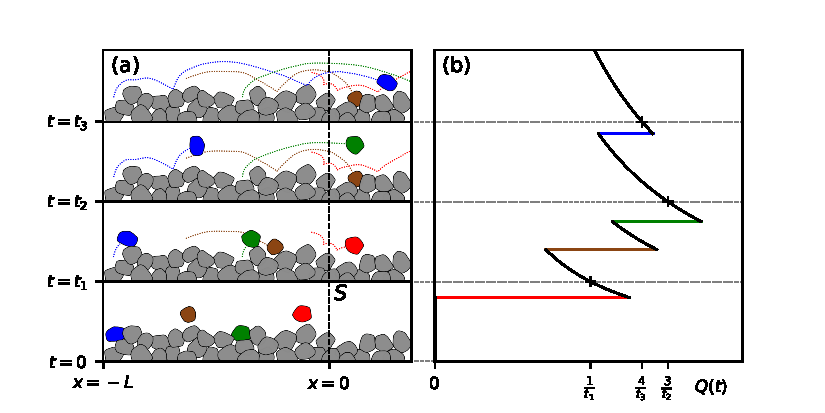
\includegraphics{./figures/ch2/figure1.pdf}}
	\caption{The left panel indicates the configuration for the flux. The particle trajectories within are calculated from equation \ref{eq:langevin}, demonstrating alternation between rest and motion with fluctuating velocity. Particles begin their transport with positions $-L\leq x \leq 0$ at $t=0$, and as depicted in the right panel, the flux is calculated as the number of particles $N_>(t)$ which lie to the right of $x=0$ at the observation time $t$, divided by $t$: $Q(t) = t^{-1}N_>(t)$. We calculate the probability distribution of $Q$ over all realizations of the trajectories and initial positions as $L\rightarrow \infty$}
	\label{fig:fig1}
\end{figure}

The rate of particles crossing the surface in an observation time $T$ is
\be Q(T) = \frac{1}{T}\sum_{i=1}^N \mathcal{I}_i(T). \ee
In this equation, $\mathcal{I}_i(T)$ is an indicator function which is $1$ whenever the $i$th particle has passed our control surface and $0$ otherwise. All particles which have not crossed the control surface (or which have crossed and then crossed back) contribute nothing to the flux. The probability distribution of the flux is then 
\be P(Q|T) = \Big \bra \delta\Big( Q - \frac{1}{T}\sum_{i=1}^N \mathcal{I}_i(T) \Big) \Big\ket. \ee
The average is over the initial conditions of each particle and the ensemble of trajectories for each particle.
Taking the Laplace transform over $Q$ (i.e. forming the characteristic function) obtains
\begin{align} \tilde{P}(s|T) &= \Bigg\bra \int_0^\infty dQ e^{-s Q}\delta\Big( Q - \frac{1}{T}\sum_{i=1}^N \mathcal{I}_i(T) \Big)\Bigg\ket \\
	&=  \Big\bra \exp\Big(\frac{s}{T}\sum_{i=1}^N \mathcal{I}_i(T)\Big)\Big\ket \\
	&=  \prod_{i=1}^N \Big\bra \exp\Big(-\frac{s}{T}\mathcal{I}_i(T)\Big)\Big\ket \\
	&= \prod_{i=1}^N \Big[1-\big(1-e^{-s/T}\big)\big\bra \mathcal{I}_i(T) \big\ket \Big] \end{align}
This progression relies on the independence of averages for each particle (so the average of a product is the product of averages) and the fact that  $ \mathcal{I}_i(T)$ is either $1$ or $0$, so that $e^{ax} = 1-(1-e^a)x$.
The average over initial conditions and possible trajectories for the $i$th particle can be written
\be \bra \mathcal{I}_i(t) \ket = \frac{1}{L}\int_L^0 dx' \int_0^\infty dx \mathcal{P}(x,t|x') =  \frac{1}{L}\int_0^L dx' \int_0^\infty dx \mathcal{P}(x,t|-x'), \ee
where $\mathcal{P}(x,t|x')$ is the probability density that the particle is found at position $x$ at time $t$ given it was initially at $x'$ at time $0$. This is the part of the flux that depends on the particle dynamics (ie instantenous velocities and entrainment/deposition characteristics).

Inserting (7) into (6) and taking the limit as $L\rightarrow \infty$ and $N \rightarrow \infty$ while the density of particles $\rho = N/L$ remains constant provides
\be \tilde{P}(s|T) = \lim_{N \rightarrow \infty} \Big(1 - \frac{1}{N}\big(1-e^{-s/T}\big)\mu(T) \Big)^N = \exp \Big[ -\big(1-e^{-s/T}\big)\mu(T) \Big].\ee
where $\mu(T) = \rho \int_0^\infty dx \int_0^\infty dx' \mathcal{P}(x,T|x')$ is a rate constant which encodes the particle dynamics. This expression is the characteristic function of a Poisson distribution \citep{Cox1965}.
Expanding in $e^{-s/T}$ and inverting the Laplace transform provides the probability distribution of the flux, contingent on the sampling time $T$:
\be P(Q|T) = \sum_{k=0}^\infty \frac{\mu(T)^k}{k!}e^{-\mu(T)}\delta(Q-\frac{k}{T}).\ee
This equation implies that the mean flux is $\bra Q \ket(T) = \int_0^\infty dQ Q P(Q|T) = \mu(T)/T$, and similarly the variance is $\sigma_Q^2(T) = \mu(T)/T^2$. 
The conclusion is that if the flux is considered as a time averaged number of particles crossing a control surface, the mean flux is always Poissonian, no matter how particles move, provided the particles are independent and do not interact.


\section{Results \label{sec:res}}
\subsection{The position probability distribution and its moments}
\begin{figure}
	\centerline{\includegraphics{figures/ch2/figure2_slopeKey.pdf}}
	\caption{Panel (a) indicates the probability distribution of particle position as it evolves through time. From the initial mixture of motion and rest states, particles advect downstream as they diffuse due to differences in their fluctuating velocities and exchange between motion and rest. Panel (b) shows the resulting particle diffusion. At timescales $t \ll 2D/V^2$, the diffusion is normal since the movement is approximately a standard diffusion process (as advection is irrelevant on these timescales). For larger timescales, $2D/V^2 \ll t \ll \tau$, particles undergo ballistic diffusion similar to \citet{Lisle1998} as a result of some particles being stationary as others advect. Finally longer than the timescale $\tau = 1/k$ associated with entrainment and deposition, diffusion is again normal, exemplified by exchange between motion and rest. All results are scaled by the mean hop length $l=V/k_D$ and the autocorrelation time $\tau=1/k$ of the motion/rest alternation.}
	\label{fig:fig1}
\end{figure}
The master equation \ref{eq:master} describes the evolution of the probability distribution of position through time. Loosely speaking the solution of this equation is expected to be some combination of the \citet{Einstein1937} theory for particle transport with the Gaussian propagator of the advection-diffusion equation \citep{Morse1953a}. 

Because the master equation is second order in time, it requires initial conditions for $P$ and $\pt P$. Considering that particles start at rest in a mixture of motion and rest states, with a fraction $k_E/k$ starting in motion and a fraction $k_D/k$ starting in rest, these conditions derive from the state 
\be P(x,0) = \lim_{t\rightarrow 0 } \frac{k_E}{k} \sqrt{\frac{1}{4\pi D t}} \exp\Big[-\frac{(x-Vt)^2}{4Dt}\Big]+ \frac{k_D}{k}\delta(x)\ee
which gives $P(x,0) = \delta(x)$ and $ \pt P(x,0) = \frac{k_E}{k}\big[D\delta''(x)-V \delta'(x) \big]$ \citep{Weiss2002}.

The master equation \ref{eq:master} is solved by transform calculus in the appendix, providing
\begin{multline} P(x,t) = \big[-\varphi D\px^2 + V\varphi \px + k + \pt \big]\int_0^t \mathcal{I}_0\Big( 2 \sqrt{k_Ek_D u(t-u)}\Big) e^{-k_E(t-u)} \\ \times \sqrt{ \frac{1}{4\pi D u}} \exp\Big[-k_D u - \frac{(x-Vu)^2}{4Du}\Big] du. \label{eq:monster}
 \end{multline}
This integral term encodes the earlier expectation of Einstein model-like behavior mixed with a Gaussian propagator. The integral term convolves the probability that the particle has been in motion for a period $u$ out of a time $t$ with the probability density that a particle has travelled a distance $x$ in time $u$. The prefactor involving partial derivatives can be understood as adapting this distribution to the initial conditions.

The moments of position from this distribution could be calculated by integrating equation \ref{eq:monster}, but this is challenging. Instead, we calculate the governing equation of the moments directly from the master equation \ref{eq:master}. Multipling this equation by $x^l$ and integrating over all $x$ provides
\be \pt^2 m_l -V l \pt m_{l-1} -k_E V l m_{l-1} + k \pt m_l - D l (l-1) \pt m_{l-2} - k_E D l(l-1) m_{l-2} = 0,\ee
where $\bra x^l \ket = m_l$. 
For $l = 1$, this equation generates the mean position $ \bra x \ket(t) = k_E V t/k$, which is unaffected by diffusion (since Gaussian velocity fluctuations are symmetric).
The case $l=2$ provides the second moment, which provides the variance of position
\be \sigma_x^2 = \frac{2k_Ek_DV^2}{k^3}\Big( t + \frac{1}{k}e^{-k t} - \frac{1}{k}\Big) + 2\frac{k_E D}{k}t.\ee
At short times $t\ll k^{-1}$, this becomes
\be \sigma_x^2 \sim \frac{k_E k_D V^2}{k^2} t^2 + \frac{2 k_E D }{k}t,\ee
so it scales as $\sigma_x^2 \sim t^2$ when $t \gg \frac{2Dk}{V^2 k_D}$ and $\sigma_x^2 \sim t$ when $t \ll \frac{2Dk}{V^2 k_D}$.
Similarly at long times $t\gg k^{-1}$, 
\be \sigma_x^2 \sim \frac{2k_Ek_D V^2}{k^3}t,\ee
so we have a non-trivial multi-scale diffusion phenomenon. 
Provided that $2D/V^2 \ll k_D/k^2$, we therefore have
\be \sigma_x^2 \sim 
\begin{cases}
	 t, & t \ll \frac{2Dk}{V^2 k_D}, \\ 
	 t^2, &  \frac{2Dk}{V^2 k_D} \ll t \ll \frac{1}{k}, \\
	 t, & t\gg \frac{1}{k}.
\end{cases}\ee
Note in the physical condition when $k\approx k_D$, the condition for the existence of three ranges becomes $ \Pe \ll 1,$ where
$\Pe = 2 D k_D/V^2.$
The small Peclet limit, when three diffusion ranges are obtained, is characteristic of bedload sediment transport where velocity fluctuations are typically small compared to mean downstream movement velocites. 

\subsection{Calculation of the sediment flux}

From the formalism in section xxxx, the central parameter of the sediment flux distribution is 
\be \mu(t) = \rho \int_0^\infty dx_i \int_0^\infty dx P(x+x_i,t).\ee
This represents the rate of particles crossing $x=0$ at the observation time $T$ given they started somewhere to left of $x=0$ at $T=0$.

It is convenient to calculate this quantity in Laplace space.   
Taking the Laplace transform,
\be \tilde{\mu}(s) = \rho \int_0^\infty dx_i \int_0^\infty dx \tilde{P}(x+x_i,s),\ee
then performing both integrals provides
\be  \tilde{\mu}(s) = -\frac{\phi D}{V R(s+k_E)} + \frac{2D\phi}{VR(1-R)(s+k_E)} + \frac{4D^2(s+k)}{V^3R(1-R)^2(s+k_E)}. \label{eq:laplacefluxrate}\ee
$\mu(t)$ derives as the inverse Laplace transform of this equation. 
This calculation is performed in the appendix, providing
\begin{multline} 
\mu(t) = \int_0^t \mathcal{I}_0\Big(2\sqrt{k_Ek_Du(t-u)}\Big)e^{-k_E(t-u)-k_D u} \\
\times \Bigg[\sqrt{\frac{D}{\pi u}}\Big([\cev{\partial_t} + k]u-\frac{k_D}{2 k}\Big)e^{-V^2 u/4D} + \frac{V}{2}\Big([\cev{\partial_t} + k]u -\frac{k_D}{k}\Big) \erfc\Bigg(-\sqrt{\frac{V^2 u}{4D}}\Bigg)\Bigg] du. \label{eq:fluxy}
\end{multline}
In this equation, the notation $\cev{\partial}$ means that the derivative acts from the left of all terms in which it is involved, as in $f(t)\cev{partial}_t g(t) = \partial_t f(t)g(t).$

This is a complicated result for the rate constant in the sediment flux \ref{eq:fluxdist}, but this complexity is not surprising given that equation \ref{eq:langevin} involves two interacting diffusion processes. As displayed in \ref{fig:fig3}, as a result of eq. \ref{eq:fluxy} the mean flux takes on a non-trivial scale-dependence, characterized by a decay toward the Einstein prediction $Q_0 = E l$ as the observation time becomes much larger than $1/(k_D \Pe)$. 

\begin{figure}[!htbp]
	\includegraphics[width=\linewidth,keepaspectratio]{figures/ch2/figure3_slopeKey.pdf}
	\caption{}
	\label{fig:fluxconvergence}
\end{figure}
The convergence time of the flux thus scales with the inverse Peclet number. When particle velocity fluctuations during motions are larger compared to advection, the flux becomes slow to converge, in general. 

\subsection{Reduction to earlier work}

The mathematical form of our results is complicated, although the ideas are conceptually clear. Particles alternate through motion and rest, and particle motions have a fluctuating velocity, not a deterministic velocity. 
Nevertheless, turning off velocity fluctuations by setting $D=0$ re-derives the results of \citet{Lisle1998}, who formulated sediment transport as a random walk between motion and rest states.
Further taking the velocity infinite as the time spent in motion vanishes, while their product $V/k_D = \ell$, the mean step distance, rederives the central result of \citet{Einstein1937}, given originally in \ref{eq:einsteinpdf}.

In either of these limit cases, the mean sediment flux becomes $\bra q \ket = E \ell$, with no dependence on observation scale. This indicates that scale dependence in the sediment flux is a consequence of velocity fluctuations among moving particles, at least when observation timescales are relatively short.
 
\section{Discussion \label{sec:disc}}

This chapter has generalized the earlier descriptions of individual sediment trajectories \citep[e.g.][]{Lisle1998,Lajeunesse2017} to include velocity fluctuations in the motion state. Using results from this generalized model as an example, I demonstrated how to calculate the sediment flux probability distribution, phrasing earlier renewal theory approaches more directly in terms of the underlying particle dynamics \citep[e.g.][]{Turowski2010,Ancey2020}. 
Calculated in this way, the sediment flux distribution is observation-scale dependent, describing how sediment fluxes depend on the period over which they are measured.

\subsection{Fluctuations and collective motions}

The sediment flux probability distribution in equation \ref{eq:fluxdist} represents a Poisson distribution with an observation-scale dependent rate.
Poisson distributions have a relatively thin tail, meaning fluctuations are typically small \citep{Ancey2006}.
In reality, sediment flux distributions are only Poissonian at high transport rates, whereas in other conditions they have wide tails representing the possibility of extremely large transport fluctuations \citep{Ancey2008,Turowski2010,Dhont2018,Saletti2015} which appear as bursts \citep[e.g.][]{Goh2008} in the sediment flux timeseries \citep{Singh2009, Heyman2013,Benavides2021}. This exposes a need to generalize a mechanistic theory of the sediment flux I developed here to produce wider fluctuations.

Descriptions of sediment transport based on population dynamics in a control volume have realistically-wide fluctuations by incorporating a positive feedback between the number of moving particles and the particle entrainment rate called collective entrainment \citep{Ancey2008,Ancey2014}.
This feedback generates spatially-correlated waves of moving particles \citep{Ancey2014, Heyman2015} and produces non-exponential interarrival time distributions \citep{Heyman2013} which imply wide-tailed flux distributions when incorporated in renewal theory \citep{Turowski2010,Ancey2020}.
Collective entrainment has been attributed to particle-particle interactions, such as small granular avalanches and collision-induced entrainment, and to fluid-particle interactions, such as large eddies entraining particles as they sweep downstream \citep{Heyman2014a,Ancey2014,Lee2018}.

We can imagine generalizing the description in equation \ref{eq:Langevin} to include such fluid-particle interactions by including time dependence in the movement velocity ($V$), diffusivity ($D$), or entrainment and deposition rates ($k_E$ and $k_D$) as necessary, although the resulting equations would likely require numerical solutions.
Particle-particle interactions would be more challenging to include.
The dynamical equation \ref{eq:langevin} would generalize to $\dot{x}_i(t) = F_i(x_i,t) + \sum_{i\neq j}G_{ij}(\{x_j\},t)$, where the $F_i$ are the driving terms unique to each particle, while the $G_{ij}$ are some (generally stochastic) terms representing interactions between the $i$th and $j$th particles \citep{Goldstein1997}. The resulting joint distribution of particle positions and velocities ($P(x_1,v_1,\dots,x_{N(t)},v_{N(t)},t)$) might be formulated by analogy to the theory of reaction diffusion systems \citep{Pechenik1999, Cardy2008}, non-ideal gases \citep{Chapman1970,Brilliantov2004}, or other interacting particle models available in physics literature \citep{Hernandez2004,Escaff2018}. 
By analogy to collective entrainment, interacting models which generalize the approach established in this chapter should be capable of producing wide sediment transport fluctuations.

\subsection{Measurement protocol for the sediment flux}




\subsection{Stochasticity in landscape evolution}

\citet{Exner1925} originally phrased channel morphodynamics in terms of spatial gradients in the sediment flux (sec. \ref{eq:exner}), writing
\be (1-\phi) \pt h(x,t) = -\px q(x,t). \ref{eq:stocEx}\ee
In this one-dimensional equation, $h(x,t)$ is a continuous field representing the longitudinal channel profile.
Traditionally, the Exner equation is evaluated considering the flux as a deterministic quantity \citep{Parker2007,Viparelli2011,An2017}, which provides a solitary trajectory of the profile through time.

Considering the flux in the Exner equation as a stochastic quantity requires us to reinterpret channel dynamics in a way which few researchers have explored \citep{Jerolmack2005,Bohorquez2016}.
In contrast to the traditional analysis, a stochastic Exner equation with fluctuating $q(x,t)$ generates an ensemble of possibilities for the channel profile $z(x)$ at each instant. This set of possibilities is characterized by a probability distribution $P(\{z(x)\},t)$ for each possible profile.
Mathematically, since the channel profile is a field, evaluating such a probability distribution of channel profiles would require statistical field theory \citep{Kardar2007}.
A starting point on this analysis might be $P(\{z(x)\},t) = \bra \delta[z(x,t)-h(x,t)]\ket,$ where $h(x,t)$ involves the stochastic flux $q(x,t)$ from equation \ref{eq:stocEx}.
In this equation, $\delta[f(x)]$ is a Dirac delta functional, which generalizes the delta function $\delta(x)$ from a single-valued parameter $x$ to a continuous field $f(x)$.
Such ideas are commonly applied to understand polymers and membranes \citep{Kawakatsu2001,Nelson2004}, but they have not been introduced in geomorphology.

Introducing such a description with the stochastic Exner equation would lend new mathematical language to the old unsolved problem in geomorphology: how does variability affect landscape evolution?
Early process-based geomorphologists acknowledged variability \citep{Strahler1952,Langbein1964}, although their main efforts were to construct strategies to describe landscapes without explicitly accounting for it, producing ideas like competent conditions to summarize climatic variability \citep{Wolman1959,Wolman1978}, characteristic grain sizes to overcome sorting processes \citep{Parker1982,Andrews1983}, and averaged flow conditions to avoid flow turbulence \citep{MeyerPeter1948,Bagnold1954}.
Recent progress in stochastic approaches \citep[e.g.][]{Furbish2021a,Ancey2020b} invites us to step beyond averaged descriptions, propagate noises through the governing equations of landscape evolution, and ask with more precision to what extent fluctuations shape Earth's surface.

\section{Summary and Conclusion \label{sec:conc}} 
 
This chapter introduced a two-noise stochastic dynamical equation to describe individual bedload trajectories for particles alternating between motions and rests. The motion phase was enriched to include velocity fluctuations, forming the first physical model of this type.
The probability distribution of the bedload sediment flux was calculated from these particle dynamics, and the resulting flux distribution was demonstrated to adopt scale-dependence from the underlying trajectories of individual particles. The measurement timescales over which sediment flux observations converge were expressed in terms of the mean particle movement velocity and the typical magnitude of its fluctuations in terms of a Peclet number.
 
These results generalize the bedload trajectory models of \citet{Einstein1937}, \citet{Lisle1998}, and \citet{Lajeunesse2017} to include fluctuating movement velocities, and they reframe earlier renewal models of the sediment flux probability distribution \citep{Lajeunesse2010,Ancey2020} to explicitly include the transport dynamics of individual sediment grains. They further quantify the dependence of the sediment flux on the observation scale, and provide guidance as to the measurement times required to resolve sediment transport without ambiguity, at least in simplified configurations when bedforms are absent. 
Next steps are to include interactions between particles to produce wider sediment transport fluctuations, and to evaluate the effects of sediment transport fluctuations on channel morphodynamics.




%%%%%%%%%%%%%%%%%%%%%%%%%%%%%%%%%%%%%%%%%%%%%%%%%%%%%%%%%%%%%%%%%%%%%%%%%%%%%%%%%%%%%%%%%%%%%%%%%%%%%%%%%%%%%%%%%%%%%%%%%%%%%%%%
%%%%%%%%%%%%%%%%%%%%%%%%%%%%%%%%%%%%%%%%%%%%%%%%%%%%%%%%%%%%%%%%%%%%%%%%%%%%%%%%%%%%%%%%%%%%%%%%%%%%%%%%%%%%%%%%%%%%%%%%%%%%%%%%
%%%%%%%%%%%%%%%%%%%%%%%%%%%%%%%%%%%%%%%%%%%%%%%%%%%%%%%%%%%%%%%%%%%%%%%%%%%%%%%%%%%%%%%%%%%%%%%%%%%%%%%%%%%%%%%%%%%%%%%%%%%%%%%%
%%%%%%%%%%%%%%%%%%%%%%%%%%%%%%%%%%%%%%%%%%%%%%%%%%%%%%%%%%%%%%%%%%%%%%%%%%%%%%%%%%%%%%%%%%%%%%%%%%%%%%%%%%%%%%%%%%%%%%%%%%%%%%%%
\endinput
Introducing such a description with the stochastic Exner equation would lend new mathematical language to the old unsolved problem in geomorphology: how does variability affect landscape evolution?
The classic works all acknowledge variability \citep{Leopold1952}, although one of their main efforts was to construct strategies to describe landscapes without explicitly accounting for it, producing ideas like competent flows to summarize climatic variability \citep{Wolman1960}, characteristic grain sizes to overcome sorting processes \citep{Parker1982}, or average flow energies to avoid turbulence \citep{Bagnold1954}.
Progress in stochastic approaches to river science \citep[e.g.][]{Furbish2021c,Ancey2020b} invites us to step beyond averaged descriptions, propagate noises through the governing equations of landscape evolution, and ask again with these classic works to what extent fluctuations shape Earth's surface.


This chapter upscaled from individual particle motions to calculate the sediment flux.
We can imagine going further, to upscale from the sediment flux to understand channel morphodynamics.
The sediment flux is stochastic as a result of variability in the individual particle trajectories forming it.
As a result, the channel morphodynamics should also adopt this stochasticity, although very few studies have evaluated this possibility \citep{Bohorquez2016, Jerolmack2005}.




Earlier approaches to calculate the probability distribution of the sediment flux have counted the fluctuating number of particles in a control volume with population models \citep{Ancey2008,Ancey2014}, or they have evaluated the average rate of particles crossing a control surface using the interarrival time distribution of particles from upstream \citep{Turowski2010,Ancey2020,Heyman2013}, in what is basically an application of renewal theory \citep{Cox1962}.
These approaches can be described as ``kinematic", in that they do not explicitly account for the trajectories of individual particles as they move downstream.

Here, I have demonstrated how to describe the sediment flux probability distribution from a dynamical perspective, rather than a kinematic one, using stochastic dynamical equations to describe the downstream trajectories of individual grains (eq. \ref{eq:langevin}.
In effect, the interarrival time distribution is replaced by the probability distributions of position for all individual particles available for motion, with their initial positions and velocities considered as random variables.
Particles moving downstream are counted as they cross the control surface, giving rise to a parameter $\Lambda(T)$, dependent on observation scale, which is analogous to the heuristic rate constant in the renewal theories that were reviewed in section \ref{sec:renewal} \citep{Turowski2010,Ancey2020}
This new description of the sediment flux from the grain scale particle dynamics, rather than characteristic kinematics derived from them, represents considerable progress toward a mechanistic understanding of sediment transport from statistical physics.

\subsection{Outlook and future research}

The phrasing of sediment fluxes the topographies they moderate as statistical quantities, having mean configurations and fluctuations, provides some context on the severe challenges encountered in predicting landscape change with deterministic equations \citep{}.
What we observe, looking at Earth's landscapes, may be a single realization, drawn from a spectrum of possibilities, whose precise form evades description. 
The stochastic perspective allows us to 

The sediment flux probability distribution in equation \ref{eq:fluxdist} represents a Poisson distribution with an observation-scale dependent rate.
Poisson distributions have a relatively thin tail, meaning fluctuations are typically small \citep{Ancey2006}. This contrasts with many bedload transport experiments with wide-tailed fluctuations \citep{Ancey2008,Heyman2016,Fathel2015}, especially for weak flow conditions near initiation of particle motion \citep{Benavides2021}, exposing a need to generalize a mechanistic theory of the sediment flux developed here to provide wider fluctuations.

There are essentially two mechanisms available by which wide fluctuations can arise \citep{Goh2008}. Both would be ultimately reflected in non-exponential interarrival times of particles \citep[e.g.][]{Turowski2010,Heyman2013}, although their origins would be unambigiously linked to the underlying particle transport mechanics.
The first possibility is to introduce correlations between particle movements \citep{Ancey2008,Heyman2013,Ancey2014}, such as might arise when turbulent flow fluctuations entrain many particles at once \citep{Cameron2020} or drive waves of high velocity particles downstream simultaneously \citep{Nino1996}. 
In a theory such as the one I presented here, this first mechanism for wide fluctuations could be described by temporally unsteady velocities, entrainment or deposition rates, or diffusion coefficients in the Langevin model \ref{eq:langevin}.
The second possibilty is to introduce interactions between moving particles, such as might result from collisions \citep{Lee2018} or wake vortices \citep{Schmeeckle2014} inducing particle entrainment, leading to collective waves of motion \citep{Ancey2014}.
Including such effects would require a many-body generalization of the Langevin and master equations \ref{eq:langevin} and \ref{eq:master}, where the probability distribution of position is promoted to a joint form $P(x_1,v_1,\dots,x_{N(t)},v_{N(t)},t)$, which is puzzling, since the number of particles $N(t)$ in the distribution fluctuates.
The model of \citet{Ancey2014} hints at this possibility, although its starting point is not a dynamical equation as in \ref{eq:master}.
Some hints as to how to generalize our work to include interactions between particles to describe wide-tailed sediment fluxes can be gleaned from literature on reaction-diffusion processes \citep{Hernandez2004,Cardy2006} and interacting gases \citep{Chapman1970,Brilliantov2004}. The further inclusion of interacting particle models into bedload transport theory would be an exciting development.

